%!TeX program = xelatex
\documentclass[12pt,hyperref,a4paper,UTF8]{ctexart}
\usepackage{homework}
\usepackage{booktabs}

%%-------------------------------正文开始---------------------------%%
\begin{document}

%%-----------------------封面--------------------%%
\cover

%%------------------摘要-------------%%
%\begin{abstract}
%
%在此填写摘要内容
%
%\end{abstract}

\thispagestyle{empty} % 首页不显示页码

%%--------------------------目录页------------------------%%
\newpage
\tableofcontents

%%------------------------正文页从这里开始-------------------%
\newpage

%%可选择这里也放一个标题
%\begin{center}
%    \title{ \Huge \textbf{{标题}}}
%\end{center}

% ==============
% =    规则    =
% ==============
\section{规则}
\begin{enumerate}[I]
    \item DDL为每周日的23:59;
    
    \item 在规定时间内不能提交作业者,零分;

    \item 没有推导过程,只列出答案者,零分;

    \item 格式混乱,无法阅读者,零分;

    \item 不懂就问,不会就学。任何经验都是后天积累的;

    \item 关于LaTeX的一切,国内外的网站都有详尽的教学视频。例:
    \begin{itemize}
        \item \href{https://www.bilibili.com/video/BV1Jy4y1p76e/?vd_source=2c0f6624843da61e86c7e8a2b75de875}{Bilibili}

        \item \href{https://www.youtube.com/watch?v=Jp0lPj2-DQA&list=PLHXZ9OQGMqxcWWkx2DMnQmj5os2X5ZR73}{YouTube}
    \end{itemize}
\end{enumerate}

\newpage

% ==============
% =    习题    =
% ==============
\section{习题}

\subsection{CRC检验}
\textbf{问:}要发送的数据为$1101011011$。采用CRC的生成多项式是$P(X)=X^4+X+1$。试求应添加在数据后面的余数。

若要发送的数据在传输过程中最后一个$1$变成了$0$,即变成了$1101011010$,问接收端能否发现?

若要发送的数据在传输过程中最后两个$1$变成了$0$,即变成了$1101011000$,问接收端能否发现?

采用CRC检验后,数据链路层的传输是否就变成了可靠的传输?

\textbf{答:}TODO

\subsection{PPP帧}
\textbf{问:}一个PPP帧的数据部分(十六进制)是 7D 5E FE 27 7D 5D 7D 5D 65 7D 5E。试问真正的数据是什么(十六进制)?

\textbf{答:}TODO

\subsection{PPP的同步传输}
\textbf{问:}PPP协议使用同步传输技术传送比特串$0110111111111100$。
\begin{itemize}
    \item 试问经过零比特填充后会变成怎么样的比特串?
    \item 若接收端收到的PPP帧数据部分是$0001110111110111110110$,试问删除发送端加入的零比特后会变成怎么样的比特串?
\end{itemize}

\textbf{答:}TODO

\subsection{CSMA/CD协议}
\textbf{问:}假定$1$km长的CSMA/CD网络的数据率为$1$ Gbit/s。设信号在网络上的传播速率为$2\times10^5$ km/s。求能够使用此协议的最短帧长。

\textbf{答:}TODO

\subsection{集线器\&交换机}
\textbf{问:}有十个站连接到以太网上。试计算以下三种情况下每一个站能得到的带宽。
\begin{itemize}
    \item 十个站都连接到一个$10$ Mbit/s 以太网集线器;
    \item 十个站都连接到一个$100$ Mbit/s 以太网集线器;
    \item 十个站都连接到一个$10$ Mbit/s 以太网交换机。
\end{itemize}

\textbf{答:}TODO

\subsection{交换机\&虚拟局域网}
\textbf{问:}以太网交换机有何特点?用它怎么样组成虚拟局域网?


\textbf{答:}TODO

\subsection{交换机\&交换表}
\textbf{问:}如图\ref{fig:3-33}所示,以太网交换机有6个端口,分别接到5台主机和1个路由器。
\begin{figure}[h!]\label{fig:3-33}
    \centering
    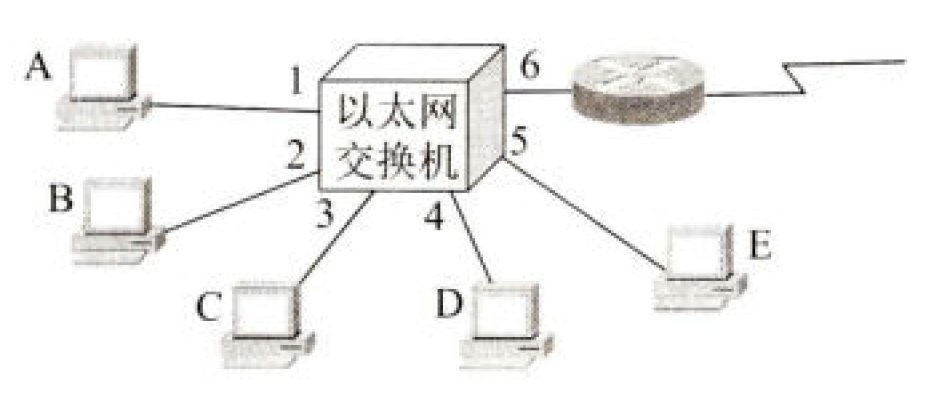
\includegraphics[width=0.5\linewidth]{figures/assignment_03_33.png}
    \caption{交换机\&交换表}
\end{figure}
在表\ref{tab:3-33}的“动作”栏中,表示先后发送了4个帧。假定在开始时,以太网交换表为空。请填写完表\ref{tab:3-33}。
\begin{table}[h!]\label{tab:3-33}
    \centering
    \caption{交换表}
    \begin{tabular}{c|c|c|c}
        \toprule
        动作 & 交换表的状态 & 向哪些端口转发帧 & 说明 \\
        \midrule
        A发送帧给D & TODO & TODO & TODO \\
        D发送帧给A & TODO & TODO & TODO \\
        E发送帧给A & TODO & TODO & TODO \\
        A发送帧给E & TODO & TODO & TODO \\
        \bottomrule
    \end{tabular}
\end{table}

\textbf{答:}TODO


\end{document}